\section{Tau lifting: the finite boundary, the global quotient of lifts,
and the original zeta
receiver}\label{tau-lifting-the-finite-boundary-the-global-quotient-of-lifts-and-the-original-zeta-receiver}

24 September 2026. Complete proofs FM0--FM7, ST0--ST10, CW0--CW7,
FA0--FA8 and FB0--FB9 follow this entry. The earlier reader, \emph{Tau
lifting and weight separation}, retains TL, WL, MT, AC and DR in full.
These two readers form successive mathematical parts; this addition does
not replace the earlier proofs.

\subsection{GL0. The controlling source and the actual
target}\label{gl0.-the-controlling-source-and-the-actual-target}

The requested target is Deligne's vanishing of an obstruction to lifting
through separation of its weights from those of the lifted classes,
proved for the user's actual tau programme. The complete preserved user
corpus and its corrections govern the operation prerequisites. In
particular, source \(Z_0\) is absence, \(0=e=\varnothing\), without
source parity; \(Z_1\) is presence \(\tau\), without \(Z_2\) parity or
addition; and the integer layer retains its amounts and \(Z_2\) data.
The withdrawn equation about adding tau is not used. No coefficient,
coordinate, weight or multiplicity below is assigned to primitive tau.

The complete global arguments consulted are corpus records
USR-9ad1c0a2d09dba92, USR-f55d16feb948d8c2 and USR-6152e3bc6302258c.
They ask for reconstruction of the entire arithmetic, globally
compatible quotients and an exact Deligne comparison. Their original
text remains in the private corpus; these descriptions are navigation,
not substitute definitions. The operation rules and individual proofs
give the relevant prerequisites before each operation. Human authorship
of the cited constructions remains with Pierre Deligne, Alain Connes,
Caterina Consani, and the other named authors.

Deligne's specialization argument uses a geometric exact sequence whose
source classes have weights at most \(i\), whereas its support
obstruction has weights at least \(i+1\). Frobenius equivariance then
forces that connecting map to vanish. The original hypotheses, duality,
Tate twist and exact sequence are retained in TL1, with the source
locators §§3.6.1--3.6.3, printed pp.~212--214. The French TeX used for
that reading is a transcription, not established original author TeX.
\href{https://www.numdam.org/item/PMIHES_1980__52__137_0/}{Deligne,
\emph{La conjecture de Weil : II}}.

The new results below construct actual receiving maps and a quotient of
their complete calculated ambiguity. They do not identify the full tau
geometric specialization with Deligne's map, and they do not assert the
requested numerical purity result as proved.

\subsection{GL1. What the retained source multiplication itself
proves}\label{gl1.-what-the-retained-source-multiplication-itself-proves}

ST starts from the current source multiplication, including its distinct
global unit \(\tau\) and integer idempotent \(1\). No source addition
involving tau is introduced. Multiplication by the already supplied
integer \(1\) gives the exact retraction \[
c:S\longrightarrow(\mathbb Z,\cdot),\qquad c(s)=1\cdot s.
\] Its sole non-singleton fibre is \(\{\tau,1\}\). This is an explicit
loss of source distinction under a map with integer input, not an
identification of source tau and integer one. ST1 proves both the
multiplicative retraction and its localization interpretation.

For a stated linear receiving action, let \(E\) be the action of integer
\(1\). Then \(E^2=E\), and ST5--ST7 prove \[
V=\ker E\oplus EV,\qquad A_n=nE\quad(n\in\mathbb Z).
\] The unit of the receiving endomorphism ring is the image of the
source global multiplicative unit; it is not assigned back to source tau
as a numerical value. The universal receiving ring, all source images
and the exact injection of the multiplicative source are constructed in
ST6. Its central idempotent separates the two receiving summands and
kills their cross-extension groups. This is a proved source-induced
splitting. It is not a computation of the numerical Frobenius weights of
the original zeta zeros.

ST also calculates the complete multiplicative prime spectrum, its
integer-additive-compatible subspace, its localizations, and its maps to
Connes--Consani's arithmetic power actions. Every operation in those
comparisons has its source, target and failure of any stronger
preservation property stated.
\href{https://arxiv.org/abs/2602.15941v1}{Connes--Consani, \emph{On the
Jacobian of Spec Z}}, as located in ST0 and ST10.

\subsection{GL2. The finite boundary changes the complete weight
calculation}\label{gl2.-the-finite-boundary-changes-the-complete-weight-calculation}

Use Connes--Consani's original action \[
\ell(a,b)(X,Y)=(aX+b,aY),
\qquad a\in\mathbb Q_{>0},\ b\in\mathbb Q,
\] on the full adelic coordinates. At each finite prime retain the
choice of Haar measure or delta at the stated coordinate. For the
two-coordinate profile \(\epsilon\), write \(d_\epsilon(p)\in\{0,1,2\}\)
for the number of delta factors at that prime. This number records
receiving distribution support; it is not the user's \(Z_2\) parity. FM1
constructs the distribution for every profile, including infinite
profiles, on the complete Schwartz--Bruhat test space. The Haar
convention \(\operatorname{vol}(\mathbb Z_p)=1\) remains explicit.

For every actual original-zeta zero \(\rho\), its actual multiplicity
\(m_\rho\), and normal order \(0\le j<m_\rho\), the full prime action is
\[
F_{p,\epsilon,j}
=p^{\rho-j+d_\epsilon(p)}
\exp\bigl((\log p)J_{m_\rho-j}\bigr).
\tag{GL2.1}
\] The archimedean normal derivative contributes \(p^{-j}\); the finite
delta factors contribute \(p^{d_\epsilon(p)}\). Neither is omitted.
FM2--FM4 prove that a nonzero all-prime intertwiner from a source zero
block \(\sigma\), normal order zero, to a target normal order \(j\)
exists exactly when \[
\rho=\sigma,\qquad
d_{\epsilon^1}(p)-d_{\epsilon^0}(p)=j
\quad\text{at every prime }p.
\tag{GL2.2}
\] The full spectral nilpotents are retained. In this Haar/delta family
a positive normal-order correction can have only \(j=1\) or \(j=2\).
This classifies the receiving family, not every possible finite-adele
distribution.

\begin{figure}
\centering
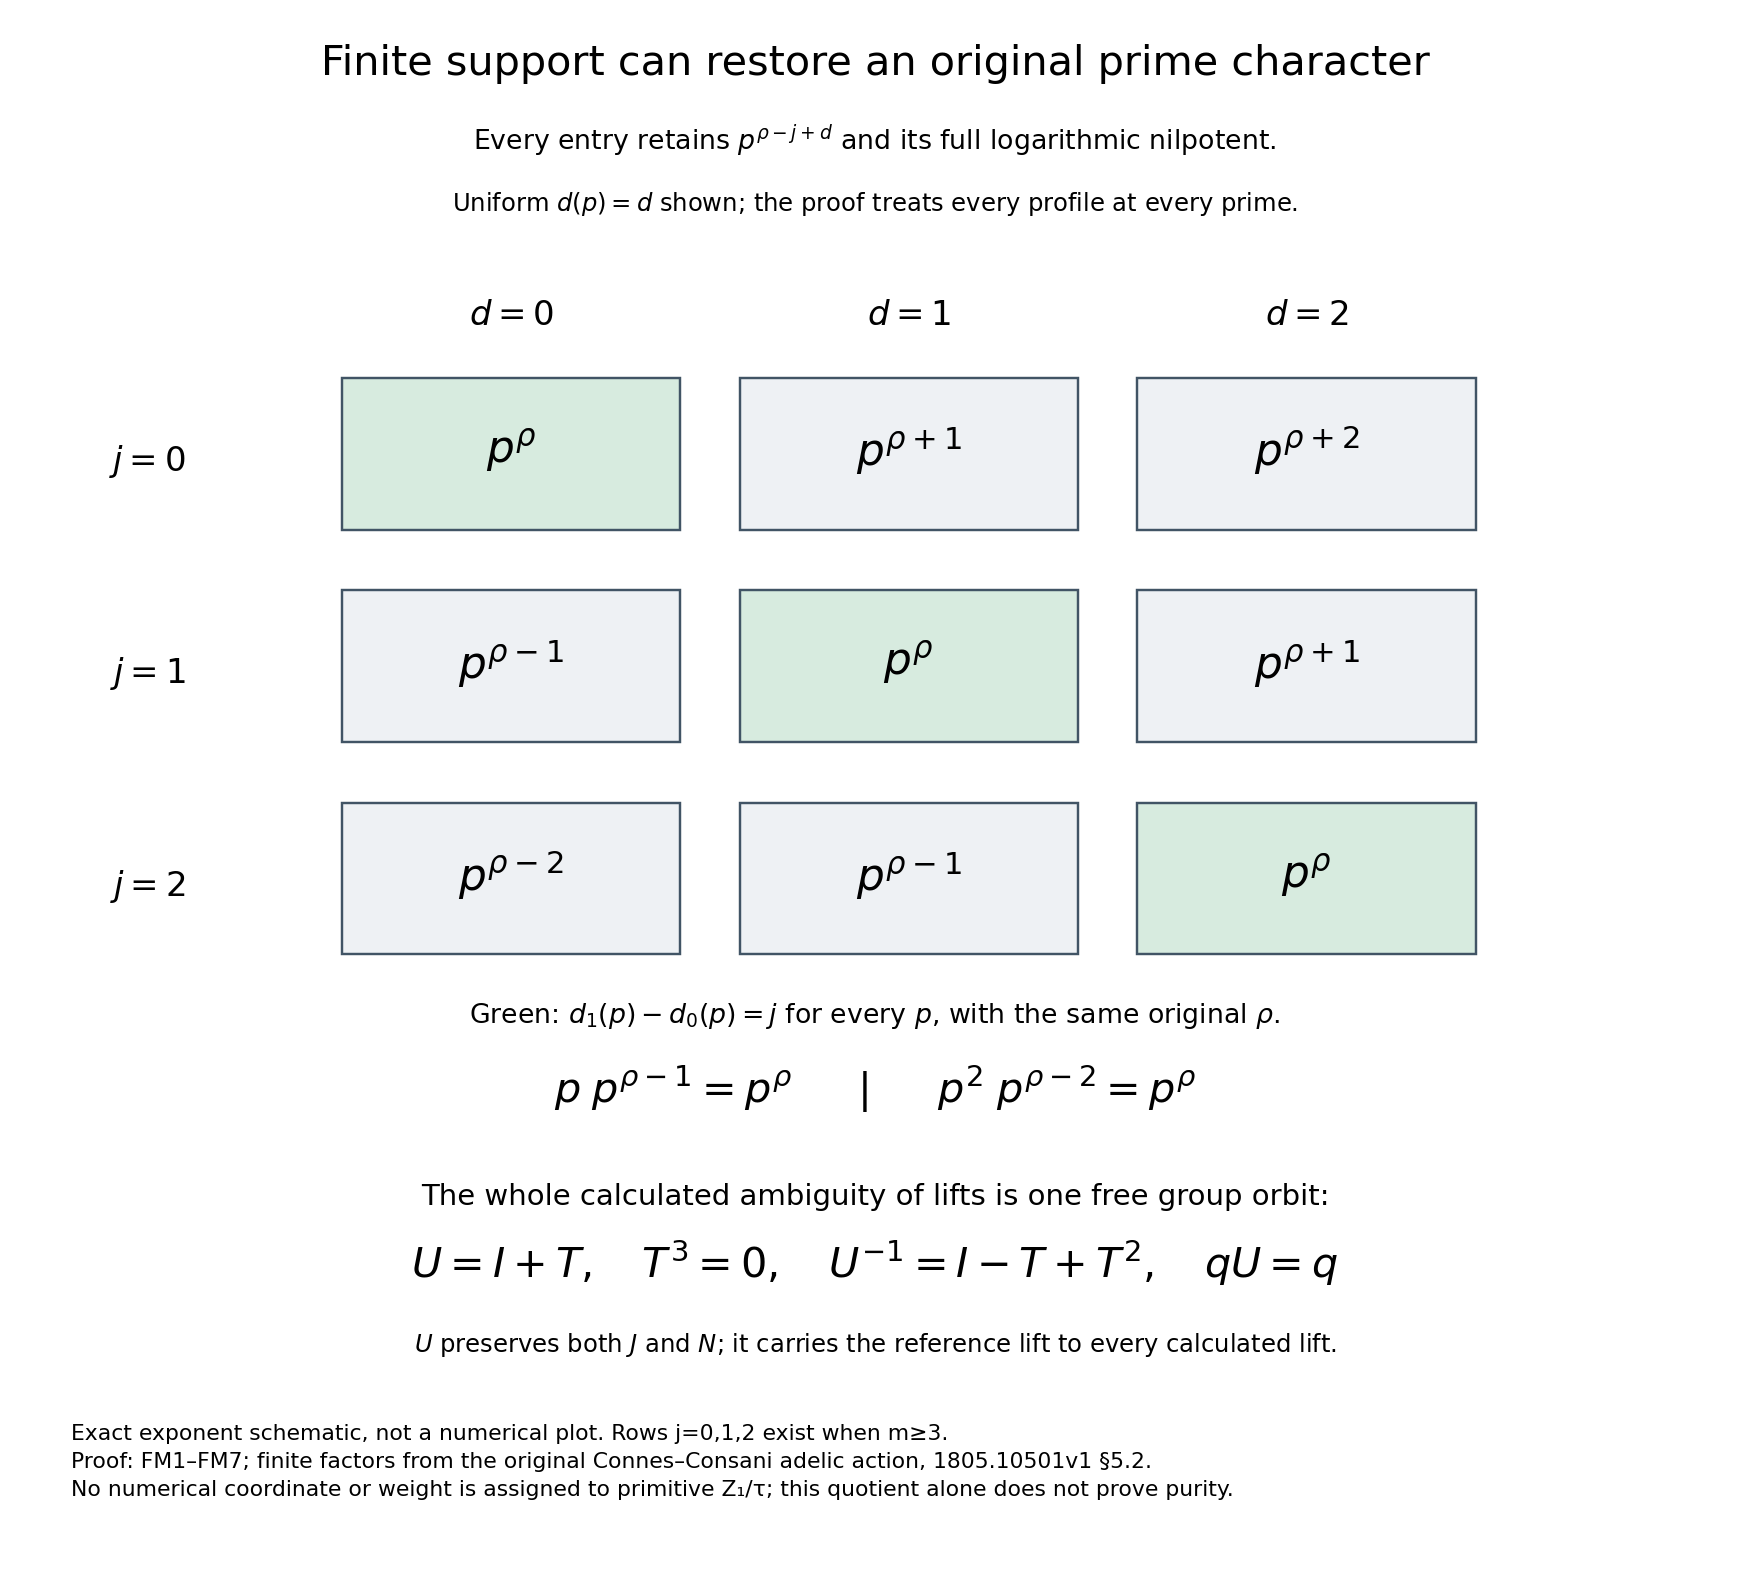
\includegraphics[width=\textwidth,height=.83\textheight,keepaspectratio]{tau_lifting_weights_20260924/FINITE_SUPPORT_LIFT_ORBIT.png}
\caption{Exact prime factors and the quotient of all calculated lifts.
The grid shows uniform profiles; FM1--FM7 prove the statement for every
profile at every prime.}
\end{figure}

Human source for the original adelic action and boundary: Connes and
Consani, §5.2, equation actionpq and Definition adelicomp2 in
\href{https://arxiv.org/abs/1805.10501v1}{\emph{The Riemann--Roch
strategy: Complex lift of the Scaling Site}}. FM and FB prove the
receiving distribution calculations rather than attributing them to that
paper.

\subsection{GL3. The whole calculated ambiguity is
quotientable}\label{gl3.-the-whole-calculated-ambiguity-is-quotientable}

Retain the exact finite algebras and map \[
B_\rho=\mathbb C[x,y]/(x,y)^{m_\rho},
\qquad A_\rho=\mathbb C[t]/t^{m_\rho},
\qquad q(x)=t,\ q(y)=0,\ i(f)=f(x).
\] Form the algebraic direct sums over all actual zeros, every receiving
profile and every rational branch, as constructed in FM7. No source tau
is an operand of their complex addition or polynomial multiplication.

FM7 proves that every section preserving the full spectral nilpotent and
the specified positive rational affine action is obtained from \(i\) by
a unique automorphism in the calculated group: \[
s=Ui,\qquad U=I+T,\qquad T^3=0,
\qquad U^{-1}=I-T+T^2,
\qquad qU=q.
\tag{GL3.1}
\] Each matrix entry of \(T\) is multiplication by \(y^jP(x)\) between
the profiles in (GL2.2). It commutes with both target nilpotents
\(J=M_x\) and \(N=M_y\), and with every stated affine action. Products
of three such entries vanish because each raises every \(d_\epsilon(p)\)
by at least one and \(0\le d_\epsilon(p)\le2\). All matrices are
column-finite, so their products and inverses exist on the algebraic
direct sum. Each entry is determined by its value at the generator \(1\)
of its receiving block; this proves uniqueness. The detailed proof,
including finite branch support and the free transitive group action, is
FM7 and its independent verification FR6--FR7.

This realizes the user's requested global quotient for this entire
family of lift differences. It preserves \(\rho\), the actual
multiplicity and the full spectral nilpotent. Consequently the quotient
of these lift differences does not itself move a zero or prove that
\(\Re\rho=1/2\). That is an exact preserved-data statement about
(GL3.1), not an objection to the user's global construction.

\subsection{GL4. The compensating term is a sheaf-local boundary
map}\label{gl4.-the-compensating-term-is-a-sheaf-local-boundary-map}

The finite trace in FB1--FB4 is \[
T_f(f)=f(X_f,0)\,dX_f\,\delta_0(Y_f).
\] Its domain is the sheaf of locally constant functions on
\(\mathbb A_f^2\), its image is the sheaf of boundary densities, and its
kernel is extension by zero from \(Y_f\ne0\). The minimal distribution
enlargement contains the regular densities and these boundary densities
as an internal direct sum. Its operator \(N_f\) sends a regular density
to \(T_f(f)\) and sends a boundary density to zero. Thus \(N_f^2=0\).
The finite product formula proves \[
P_f(a,b)N_f=aN_fP_f(a,b).
\] Together with the archimedean identity
\(P_\infty(a,b)\partial_X=a^{-1}\partial_XP_\infty(a,b)\), this gives
the actual equivariant chain map \[
\widetilde{\mathcal B}=\partial_X\otimes N_f,
\qquad \widetilde{\mathcal B}^{\,2}=0,
\qquad [\widetilde{\mathcal B},L_\lambda]=0,
\qquad L_\lambda=Y(\lambda\partial_X+i\partial_Y).
\tag{GL4.1}
\] FB5--FB6B retain the complete coefficient character \(\lambda>0\),
arithmetic Frobenius and its change \(\lambda\mapsto\lambda\mu\). In the
explicitly proved residue coordinates the induced map and the connecting
map are \[
K_\lambda=-\frac{i}{\lambda}\partial_Y\otimes T_f,
\qquad \Delta_\lambda(h)=\lambda h
\quad\text{for constant densities }h.
\tag{GL4.2}
\] The residue Frobenius includes the exact factor \(\mu^{-1}\). FB6B
proves the commutation with (GL4.2) by retaining both coefficients
\(-i/(\lambda\mu^2)\). In this specified distribution complex the
displayed connecting map is nonzero. It has not been identified with the
geometric specialization map in the requested tau theorem.

There is also a direct chain-level quotient calculation. For every
receiving complex scalar \(z\), (GL4.1) gives \[
V_z=I+z\widetilde{\mathcal B},\qquad
V_z^{-1}=I-z\widetilde{\mathcal B}.
\tag{GL4.3}
\] Multiplication gives both inverse identities because
\(\widetilde{\mathcal B}^{\,2}=0\). Commutation in (GL4.1) proves that
both maps are chain maps. The proved affine and arithmetic Frobenius
commutations give their corresponding equivariance. Projection from the
direct sum onto the original regular-density summand kills
\(\widetilde{\mathcal B}\), so this projection composed with \(V_z\) is
unchanged. Thus these transformations are invertible over that quotient
at the level of the actual stated sheaf complex, not merely a finite
matrix analogy. No assertion that this family exhausts all sheaf
automorphisms is needed or made.

\subsection{GL5. Original CC coefficients map injectively into the
original zeta
quotient}\label{gl5.-original-cc-coefficients-map-injectively-into-the-original-zeta-quotient}

CW0 constructs the entry from the original Connes--Consani constant
coefficients into their holomorphic coefficient condition. On \[
V_+=\operatorname{span}_{\mathbb C}\{[x]:x>1\}
\subset\mathbb C[\mathbb R_+^\times],\qquad
\theta_a[x]=[x^a],
\] put \(b(u)=e^{-(\log u)^2}\) and define the linear map \[
K_b[x]=W_{\log x}b,
\qquad W_a k(u)=a^{1/2}k(u/a).
\] Its original Mellin transform, including the complete nonzero factor,
is \[
F_{K_b[x]}(s)
=\sqrt\pi\,e^{(s-1/2)^2/4}(\log x)^s.
\tag{GL5.1}
\] Let \(Q=\mathcal A/\overline{\mathcal E S_{00}^{\mathrm{even}}}\) be
the original-zeta quotient, with
\(\mathcal E f(u)=u^{1/2}\sum_{n\ge1}f(nu)\) and
\(F_{\mathcal E f}(s)=\zeta(s)Mf(s)\). CW proves \[
\overline K_b:V_+\hookrightarrow Q
\] is injective and intertwines \(\theta_a\) with \(W_a\) for every
positive real \(a\). Its maps onto every finite packet of original zero
jets retain all actual multiplicities. The proof uses the full original
Mellin identity, the exact primary jets, and an unconditional count of
the original zeta zeros with multiplicity. It does not assume RH or
replace zeta by a completed function.

\begin{figure}
\centering
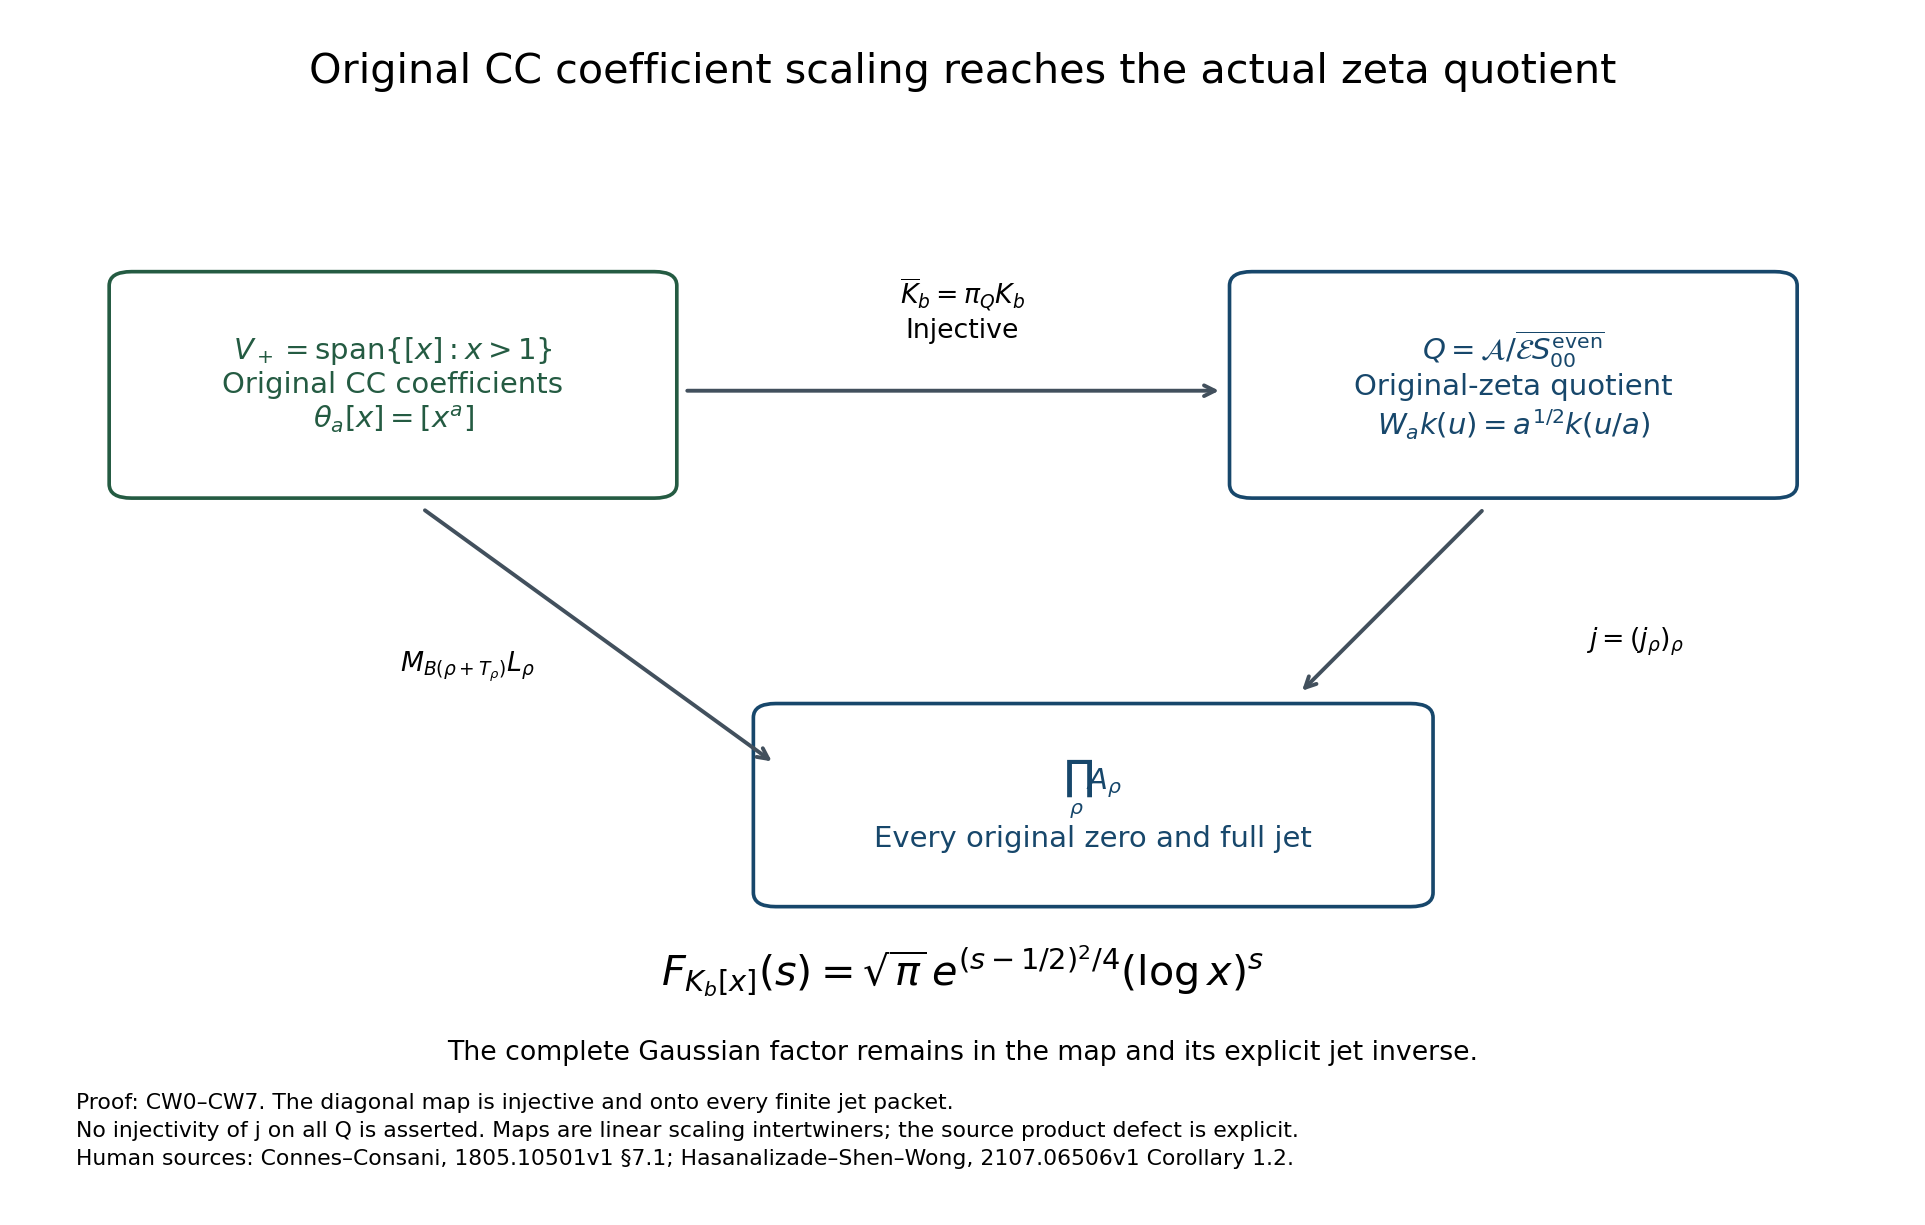
\includegraphics[width=\textwidth,height=.83\textheight,keepaspectratio]{tau_lifting_weights_20260924/CC_COEFFICIENT_MELLIN_MAP.png}
\caption{The original CC coefficient action and the full Mellin
comparison, including the Gaussian factor and every zero jet.}
\end{figure}

The global injection proof and the complete jet inverse are CW3--CW5.
CW6 calculates the failure to preserve the source algebra product and
the exact convolution identity in its place. No stronger algebra
morphism is asserted. The zero-count source is Elchin Hasanalizade,
Quanli Shen and Peng-Jie Wong,
\href{https://arxiv.org/abs/2107.06506v1}{\emph{Counting zeros of the
Riemann zeta function}}, Corollary 1.2. Its original author source
archive and the exact bounded reading coverage are preserved in the
source ledger. The coefficient construction is Connes--Consani, original
author TeX §7.1, labels holom and frobarith.

\subsection{GL6. Proof status and
continuation}\label{gl6.-proof-status-and-continuation}

The source-induced idempotent splitting, the finite-boundary chain map,
the original CC-to-zeta linear injection and the quotient of every lift
in the specified Haar/delta family are proved here. All labels, branch
coordinates, original zero multiplicities and character parameters are
retained in the full proofs. Twelve new exact symbolic matrix checks
supplement, rather than replace, the earlier 155 checks and the complete
written proofs.

The requested full tau lifting theorem remains unfinished. In
particular, the calculated quotient preserves arbitrary original zero
labels throughout the open critical strip, and the full geometric
specialization has not been proved to be the sequence whose weight
separation Deligne uses. The current calculation therefore supplies
exact maps for pursuing that identification without substituting an
auxiliary sequence or an assumed purity assertion for it.
